\setchapterpreamble[u]{\margintoc}
\chapter{Intégration}
\labch{integration}

\todoinline{
Remarques générales :
}
\todoarmand{Les trois dernières animations du chapitre "Intégration sur un intervalle quelconque" sur votre site ne sont pas accessibles, est-ce normal ?}

\todoarmand{
Inclure le flow chart \url{https://acamanes.github.io/psi/psi_doc/fc03.pdf} ? \\
J'ai vu sur votre site que vous aviez fait plein de diagrammes pour les ECT. On pourrait inclure ceux sur l'intégration ?
}

\todoarmand{J'ai modifié les différents environnements, les seules modifications par rapport aux anciens sont: "preuve" devient "demo", "elem\_demo" devient "elemdemo" et "elem\_sol" devient "elemsolution". De plus, on peut maintenant ajouter un titre optionnel entre crochets à tous les environnements: théorème, proposition, ..., exercice, remarque, démonstration, ...}

\begin{figure}[H]
    \centering
    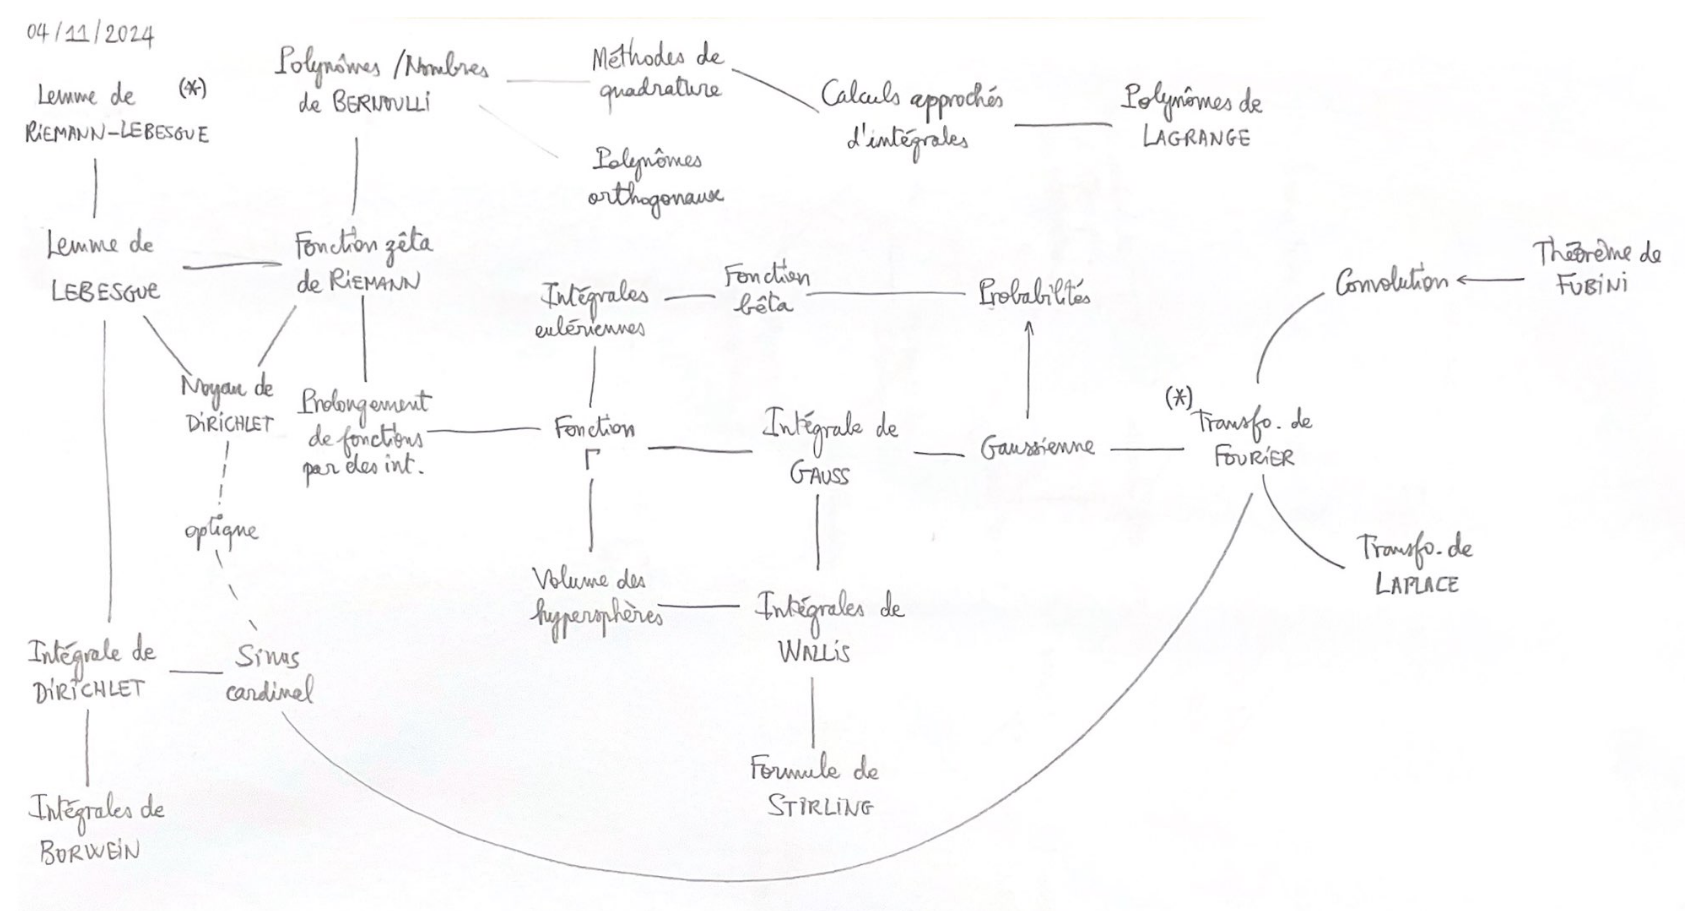
\includegraphics[width=1\linewidth]{chapitres/integration/documents/diagramme_integration.png}
    \caption{Ébauche d'un diagramme des chapitres}
\end{figure}